\section{Theoretische Grundlage}
\label{sec:Theorie}
Ziel des Versuches ist es die Totzeit, die Nachentladung sowie Charaketristik eines Geigermüllerzählrohr zu bestimmen.

\subsection{Aufbau eines Geiger-Müller-Zählrohr}
Ein Geiger-Müller-Zählrohr ist ein Messgerät zur Bestimmung von Ionisiernder Strahlung. Ein Modell eines Geiger-Müller-Zählrohr ist in Abbildung \ref{fig:skizze} zu sehen. 
\begin{figure}
  \centering
  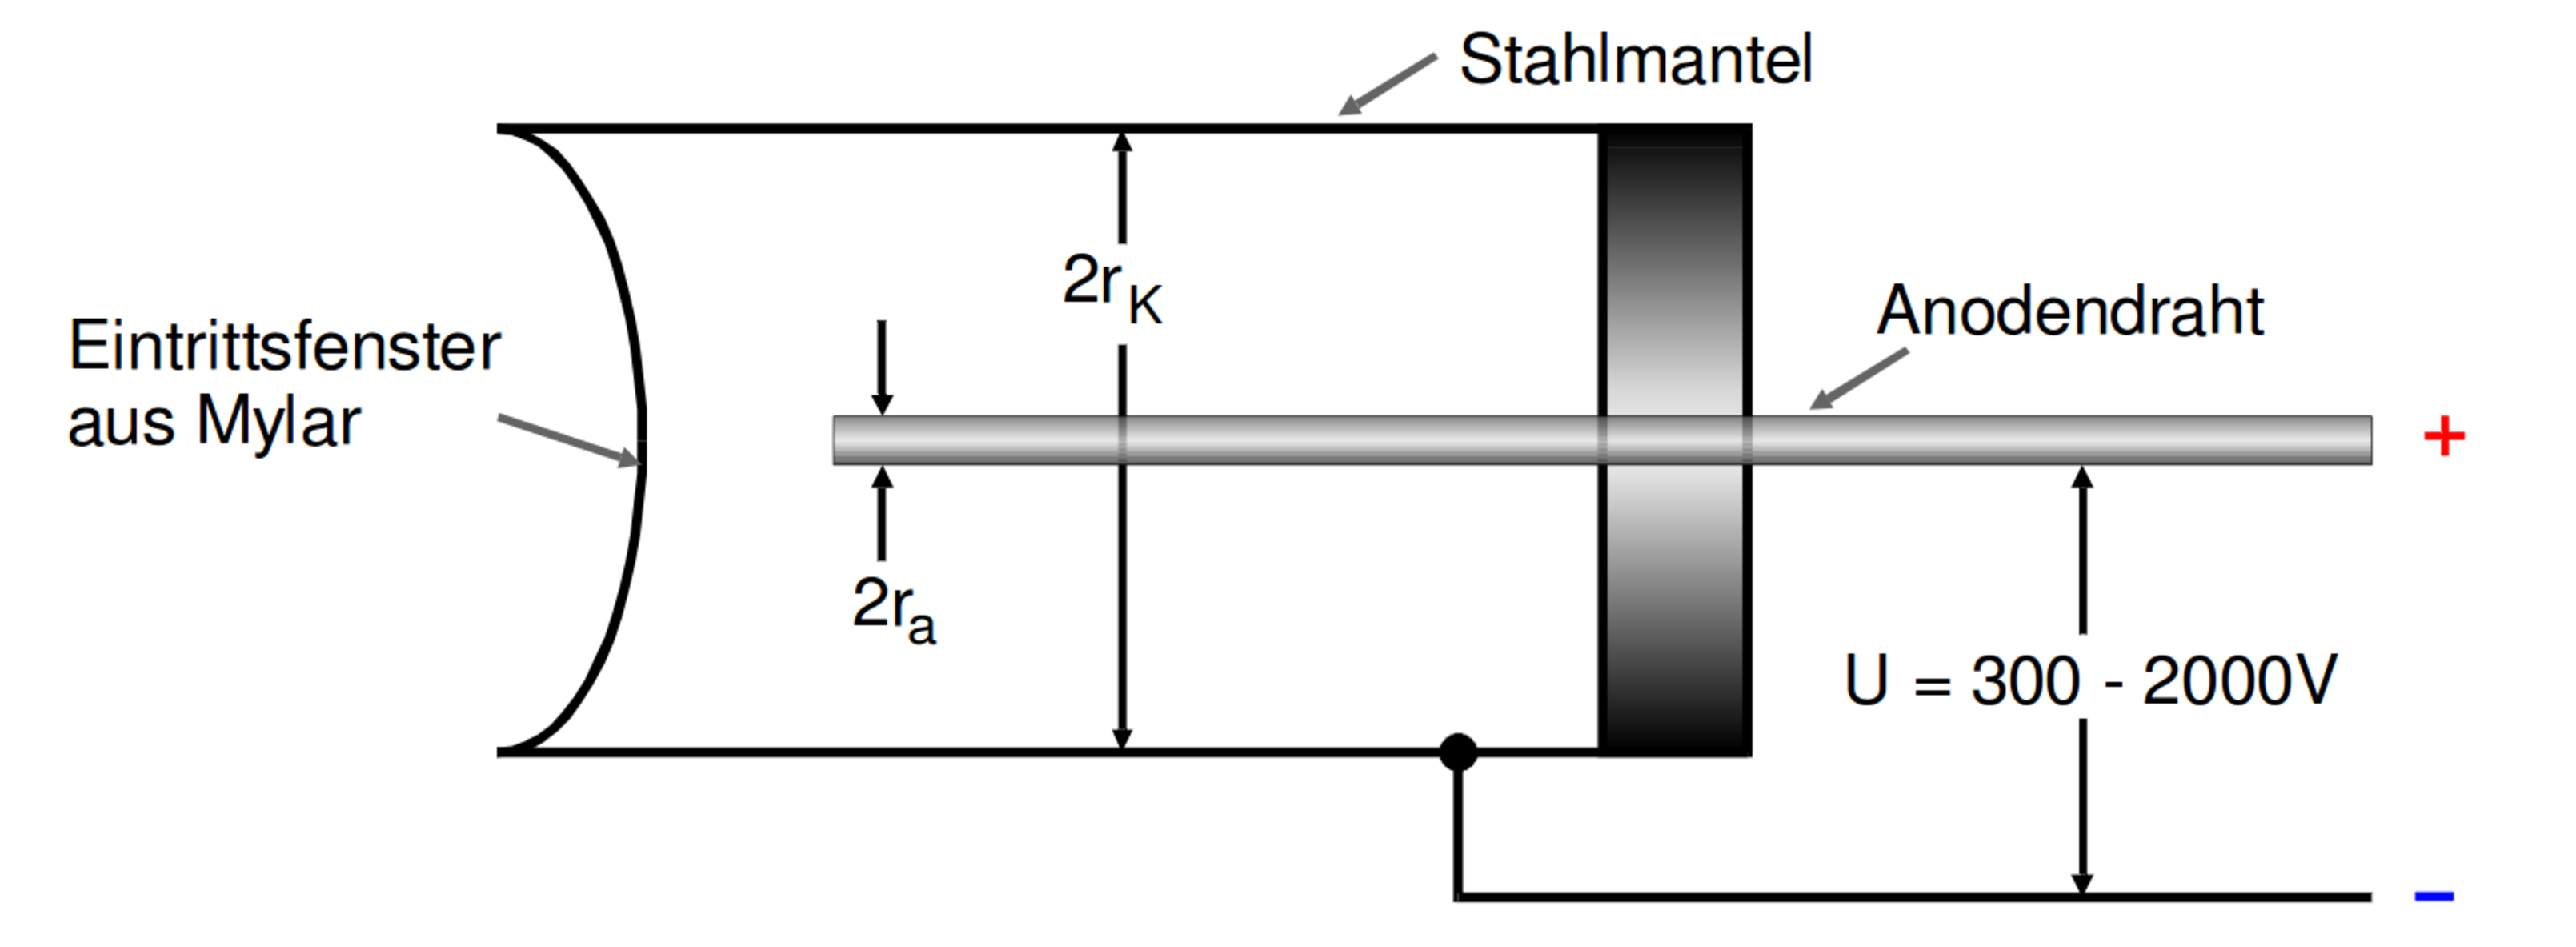
\includegraphics[height=4cm]{picture/Skizze.pdf}
  \caption{Aufbau eines Geigermüllerzählrohr \cite{sample}}
  \label{fig:skizze}
\end{figure}
Zwischen dem Anodendraht und dem Stahlmantel wird eine äußere Spannungangelgt, wodurch eine radialsymetrisches Feld zwischen Annodendraht und Kathode entsteht, deren Feldstärke 
\begin{equation}
  E(r) = \frac{U}{r ln \frac{r_\text{k}}{r_\text{a}}}
  \label{eqn:feld}
\end{equation}
beträgt. Der Stahlzilinder ist mit einem Gasgemisch aus Argon und Etyhlakohol gefüllt und wird Mylar-Folie verschlossen. Die beimischung des Alkohols soll die Nachentladung auf welche im weiteren Verlauf noch weiter eingegangen wird unterdrücken werden. Durch die Wahl von Mylar-Folie als Stirnfenster soll die Abschirmung von $\alpha$ verhindert werden und diese somit für das Geiger-Müllerzählrohr messbar seien.

\subsection{Wirkungsweise des Geigermüllerzählrohr bei unterschiedlichen Spannungen}
Beim eintreffen von Ionisierder Strahlung in das Geiger-Müller-Zählrohr werden entlang der Teilchenbahn soviel Gasatome ionisiert, bis die Teilchenenergie der Größenordnung von 100keV in Ionisierungsenergie der Atome umgewandelt ist. Somit besteht eine Proportionalität zwischen der Energie der eintreffenden Strahlung und des gemessenen Stroms. Je nach angelgeter Spannung können verschieden effekte im Zählrohr beobachte werden wie in Abbildung \ref{fig:Geb} dargestellt ist. 
\begin{figure}
  \centering
  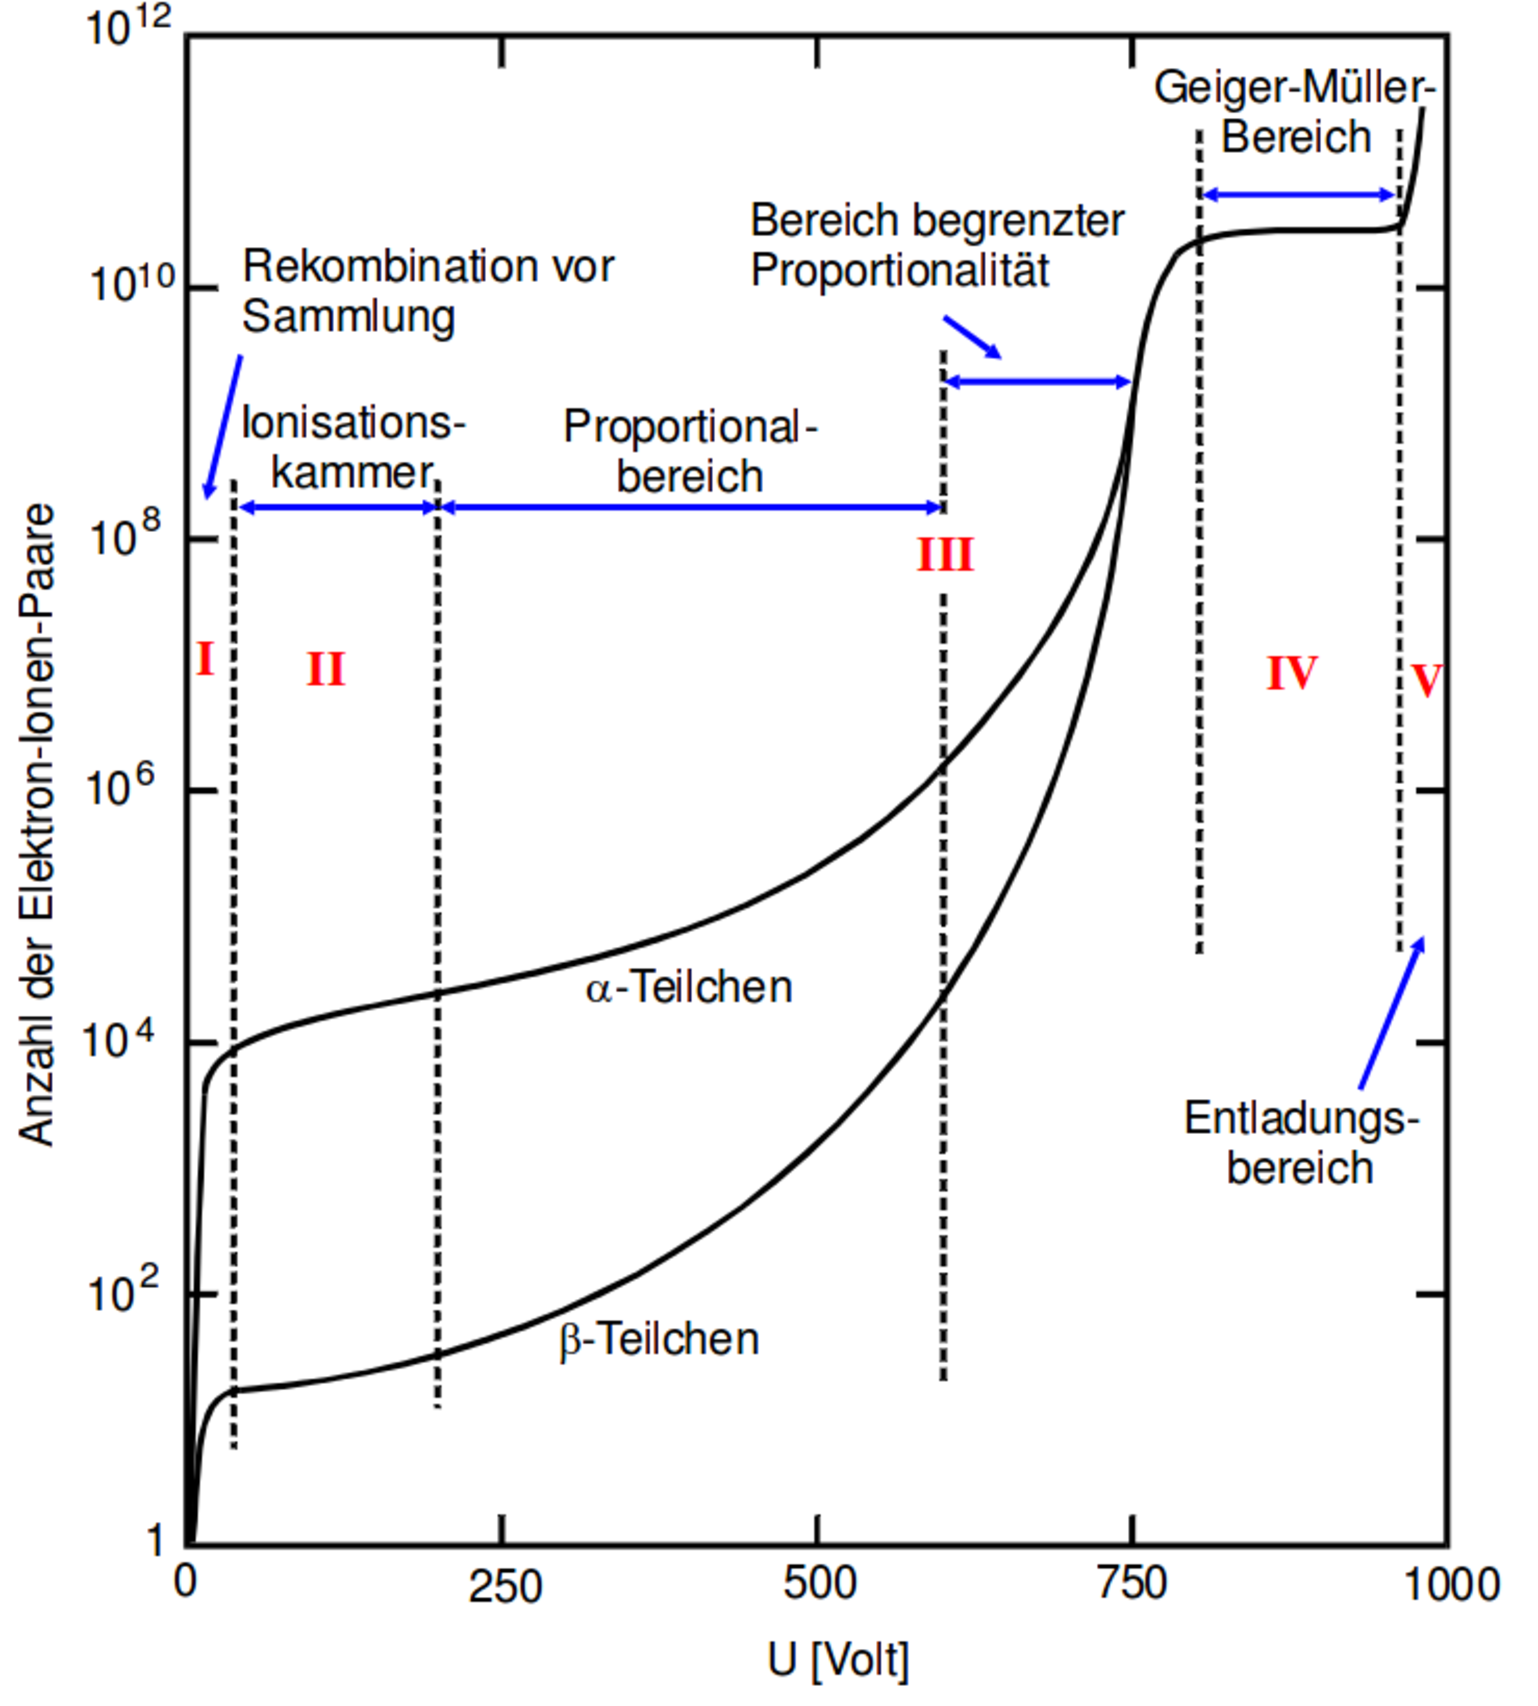
\includegraphics[height=7cm]{picture/Gebiete.pdf}
  \caption{\cite{sample}}
  \label{fig:Geb}
\end{figure}
Wird nun eine sehr kleine Zählrohrspannung $U$ angelegt rekombiniert ein Großteiel der Ionisierten Atome sich wieder bevor die Elektronen den Draht erreichen (siehe Gebiet I). Wird die Zählrohrspannung weiter erhöht, kann ein Ionisationsstrom zwischen den Kondensatorplatten gemessen werden, welcher Proportional zur Energie, sowie auch der Intensität der Ionisierenden-Strahlung ist. In Abbildung \ref{fig:Geb} ist diese Gebiet mir einer roten II gekennzeichnet. Wird die Spannung weitere gesteigert, erhalten die freigesetzten Elektronen durch das Radialsymmetrische Feld so viel kinetische Energie das diese auf den Weg zur Anode durch Stöße zusätzliche Argon Atome ionisieren. Dieses Phönomen wird als Townsend-Lawine bereichnet. Dieser Bereich (III) wird als Proportionalberreich bezeichnet und eignet sich besonders gut um die Teilchenenergie zu bestimmen, da ein hinreichend großer Strom gemessen werden kann, der proportional zur Teilchenenergie ist. Im Bereich IV wird die Spannung weiter erhöht so, dass die Elektronen einerseits beim Auftreffen auf die Argon Atome sie diese Einerseits Ionisieren als auch Anregen. Die daraus entstehenden Photonen ionisieren daraufhin im Gegensatz zu den Elektronen nicht nur Atome in Feldrichtung sondern Atome im gesamenten Zylindermantel. Es kommt zu einer primären Elektronenlawine im gesamten Zählrohrvolumen. Dies hatt zur Folge das keine Aussage mehr über die Energie der Strahlung getroffen werden kann, lediglich über die Intensität. Wenn die Kinetische Energie der Ionen groß genug wird lösen diese beim auftreffen auf den Zählrohrmantel sekundär Elektronene aus und es kommt zu einer Nachentladung. Auf den Aspekt der Nachentladung wird in den folgenden Kapiteln noch eingegangen.

\subsection{Totzeit} 
Aufgrund der wessentlich größreren Masse der Ionen im Gegensatz zu den Ionen ist deren Trägheit größer. Somit brauchen die Ionen eine wesentlich längere Zeit bis sie wieder neutral geladen sind. In dieser Zeit bauen diese einen Ionenenschlauch auf, welcher die Feldstärke soweit herabsetzt das es in der Zeit $T$ nicht mehr zu Stoßionisation kommt. In dieser Zeit kann also keine Ionisierende Strahlung mehr nachgewiesen werden. Anschließend an die Totzeit sind die Elektrischen Impulse zunächst geringer als der Primärimpuls wie in Abbildung \ref{fig:tot} zu sehen ist. Die Zeit bis die kompletten Ionen abgebaut sind wird Erholungszeit $T_\text{E}$ genannt. 
\begin{figure}
  \centering
  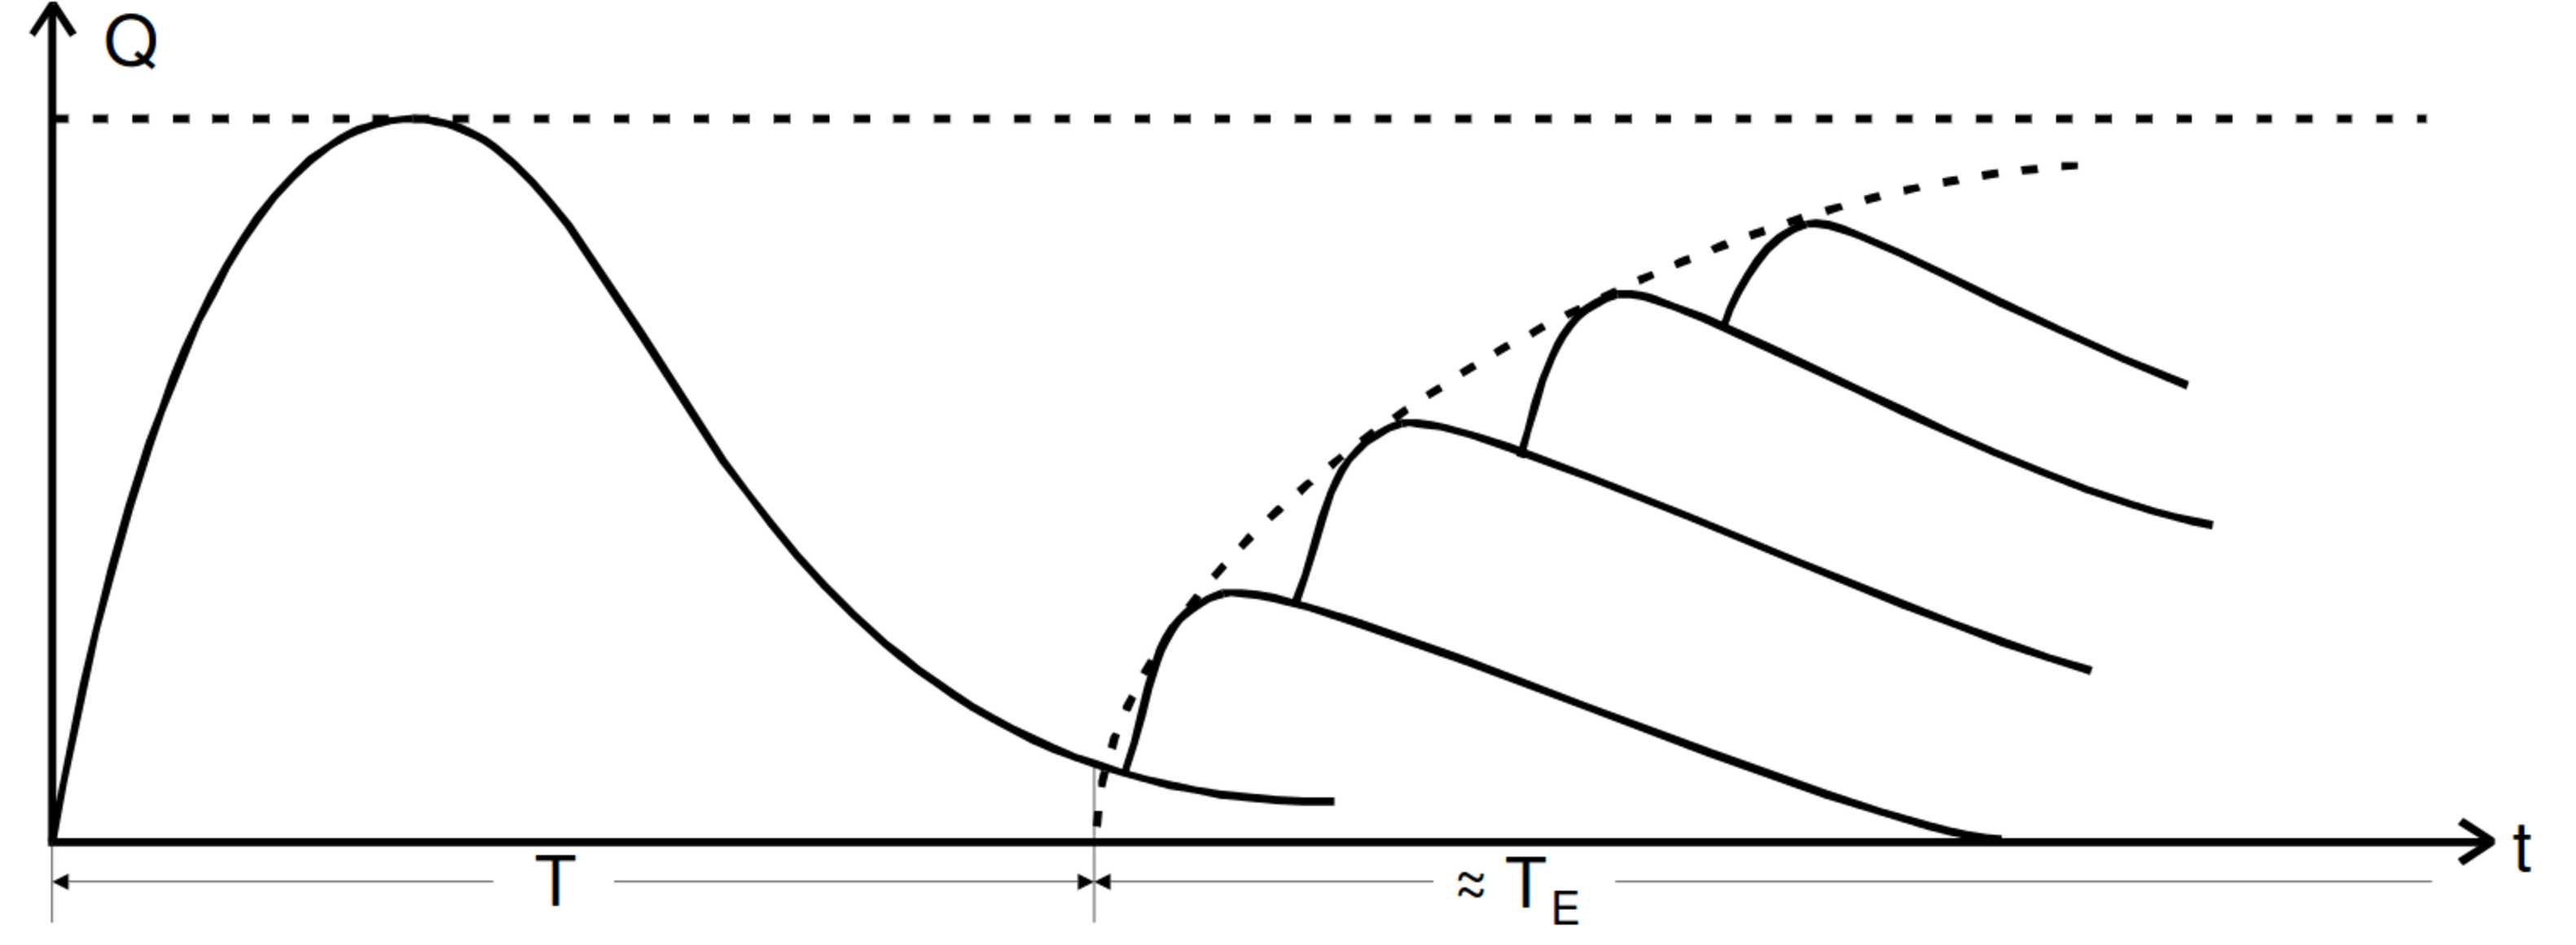
\includegraphics[height=5cm]{picture/Nachentladung.pdf}
  \caption{Tot- und Erholungszeit des Geigermüllerzahlrohrs \cite{sample}}
  \label{fig:tot}
\end{figure}

\subsection{Nachentladungen}
Wenn die Ionen durch das E-Feld hinreichend viel kinetische Energie gewinnen kann es seien, dass diese beim auftreffen auf die Mantelfäche wiederum Elektronen aus dieser Herauslösen. Dies ist Ausgangsimpuls von einer neuen Elektronenlawine. Um dies zu verhinden wird dem Gas Alkohol beigemischt, auf welches die Ionen stoßen und so ein Teil ihrer Kinetischen Energie verlieren um so mit einer niedrigeren Geschwindigkeit auf den Stahlmantelzu treffen und keine Elektronen mehr raus zu lösen. 

\subsection{Charakteristik des Zählrohrs}
Unter der Charakteristik eines Zählrohrsversteht wird das Plateau gemeint, das sich ausbildet wenn die registrierte Teilchenzahl $N$ gegen die Zählrohrspannung $U$ bei Konstanter Intensität aufgetragen wird. Ein Schema ist in Abbildung \ref{fig:Pla} zu sehen. 
\begin{figure}
  \centering
  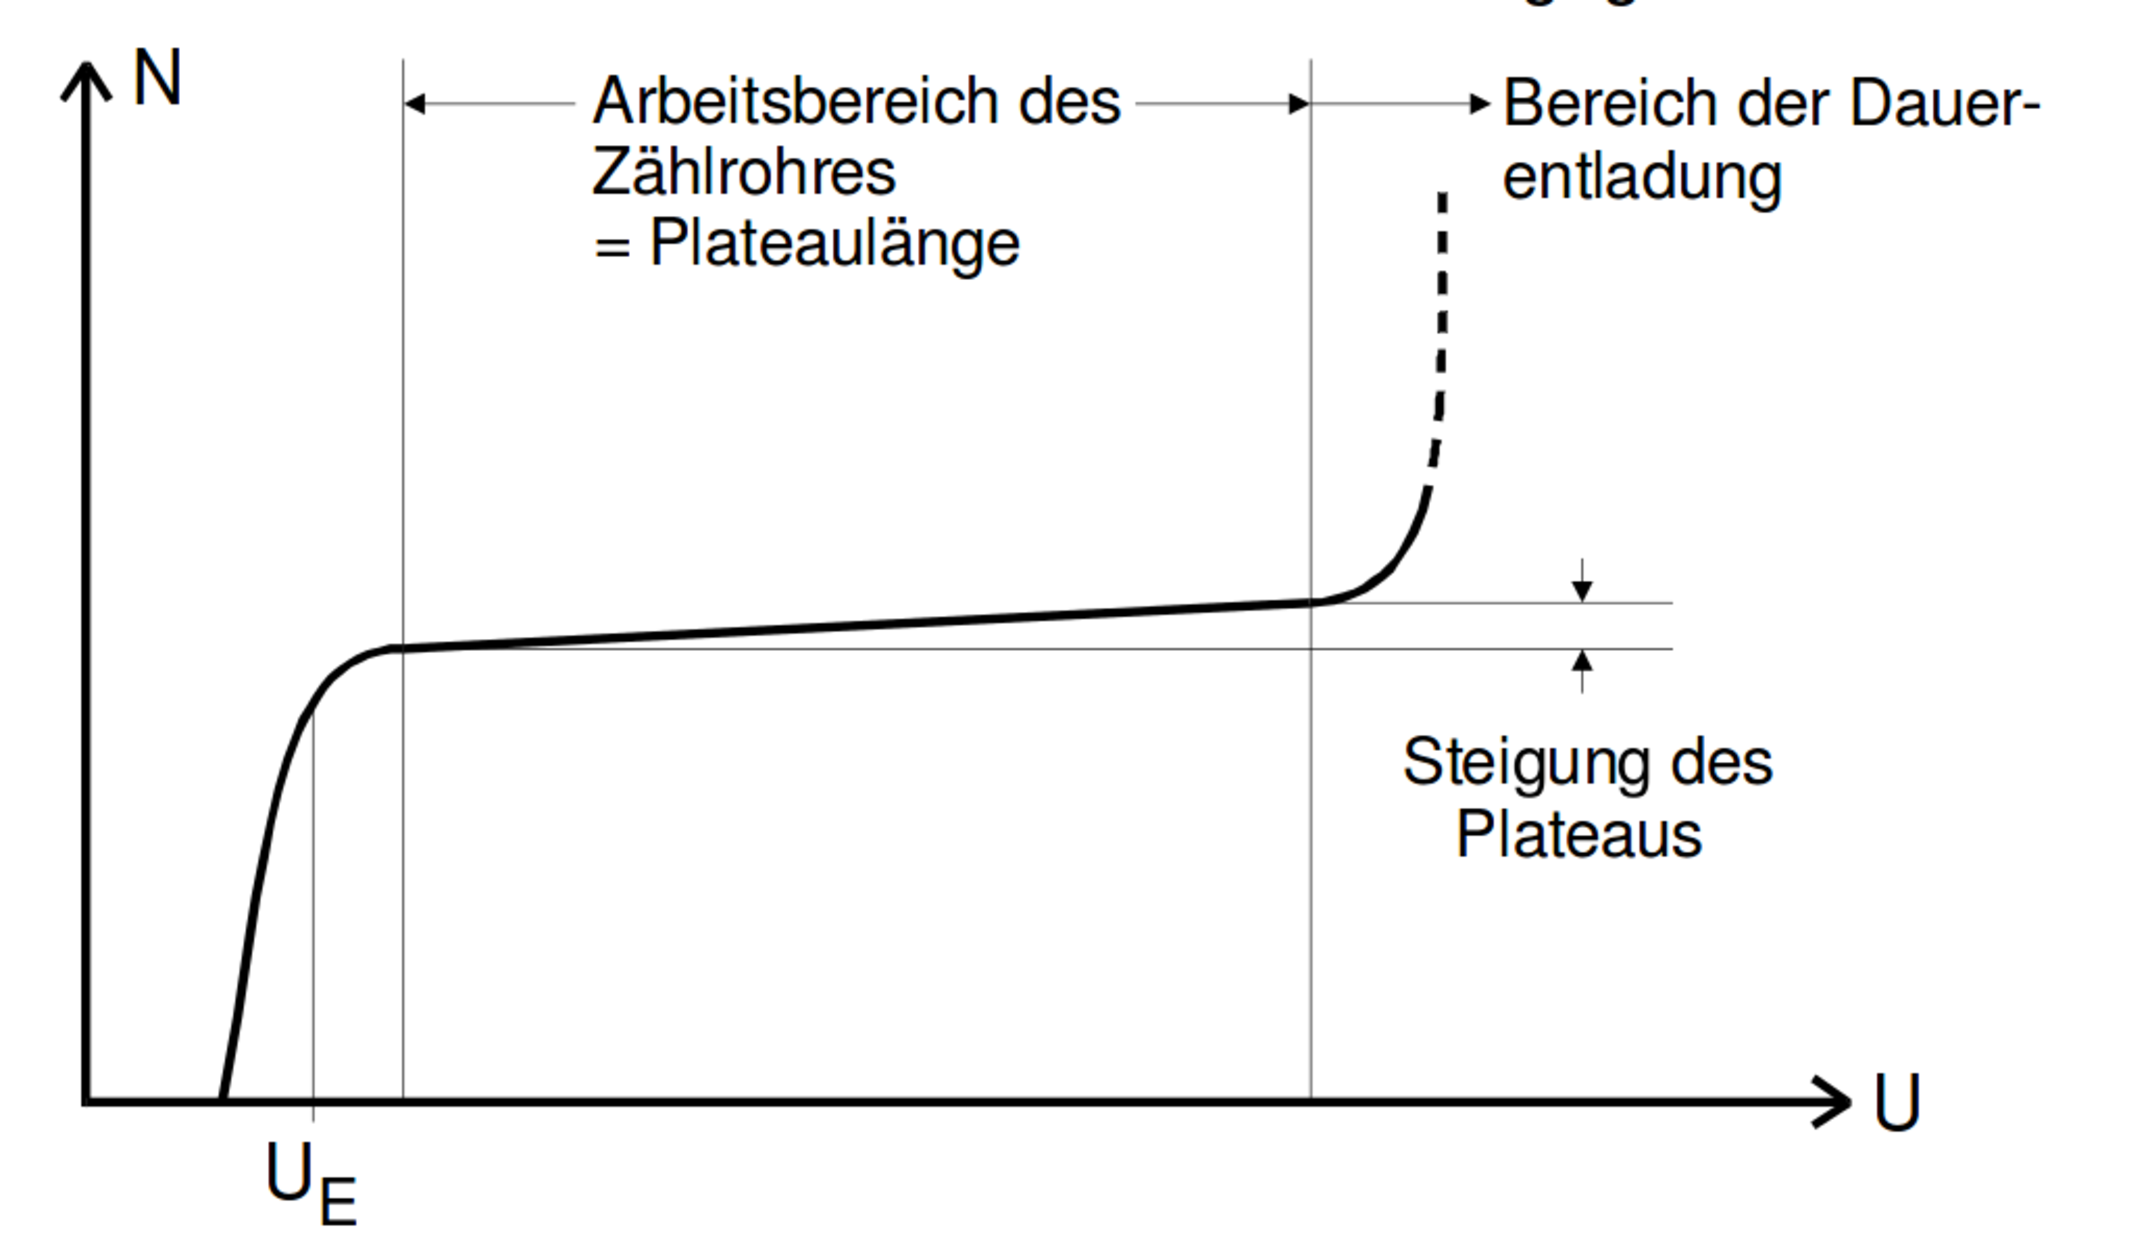
\includegraphics[height=5cm]{picture/Plateau.pdf}
  \caption{<+caption text+>}
  \label{fig:Pla}
\end{figure}
Aufgrund der Nachentladung weist der Graph eines Geiger-Müller-Zählrohr im Gegensatz zum idealen eine Steigung des Plateaus auf welche der Nachentladungen geschuldet ist. Eine geringe Steigung spricht für ein qualitativ hochwertiges Geiger-Müller-Zählrohr.

\subsection{Bestimmung der Totzeit mit der Zwei-Quellen-Methode}
Aufgrund der Totzeit des Geigermüllerzählrohr wird das Phänomen beobachtet das die Summe der Impulsrate von zwei Präperaten ($N_1 + N_2$) größer, als wenn beide Präperate ($N_{1+2}$) gleichzeitig auf das Geiger-Müller-Zählrohr gerichtet werden, ist.
\begin{equation}
  	N_1 + N_2 > N_{1+2}
  \label{eqn:ungl}
\end{equation}
Wird nun aus der Messung dedektierten Impulse $N_\text{r}$ berücksichtig das die Zählrate $N_\text{w}$ für den Momment der Totzeit $T$ keine Strahlung registiert ergibt sich die Gleichung
\begin{equation}
  N_\text{w} = \frac{N_\text{r}}{1 - T N_\text{r} } \ .
  \label{eqn:zaelr}
\end{equation}
Aus der Forderung das im Mittel aus der Summe, als auch wenn beide Prääperate gleichzeitig auf das Geiger-Müller-Zählrohr gerichtet ist, genausoviele Impulse dedektiert werden sollen, ergibt sich die Gleichung
\begin{equation}
  \frac{N_{1+2}}{1-TN_{1+2}} = \frac{N_{1}}{1-TN_{1}} + \frac{N_{2}}{1-TN_{2}} \ .
\end{equation}
Durch umstellen der Gleichung nach $T$ lässt sich anhand der Messgrößen $N_1, N_2, N_{1+2}$ näherungsweise bestimmen.
\begin{equation}
  T ~ \frac{N_1 + N_2 + N_{1+2}}{2 N_1 N_2}
  \label{eqn:T}
\end{equation}
\subsection{Fehlerrechnung}
Sämtliche Fehler und Fehlerfortpflanzungen werden mit Hilfe des Paketes "uncertainties" \cite{uncertainties} aus Python berechnet. Mit ausnahme des Fehlers der Zählrate, dieser wird über
\begin{align*}
	\Delta N = \frac{\sqrt{n_\text{Impulse}}}{\Delta t}
\end{align*}
berechnet. \\
Sämtliche Fits werden mit Hilfe der Paketes "lmfit" \cite{lmfit} aus Python berechnet.
